\documentclass[10pt,aspectratio=169]{beamer}

% silence some Metropolis warnings
\usepackage{silence}
\WarningFilter{beamerthememetropolis}{You need to compile with XeLaTeX or LuaLaTeX}
\WarningFilter{latexfont}{Font shape}
\WarningFilter{latexfont}{Some font}

% define custom colors
\usepackage{xcolor}
\definecolor{dark gray}{HTML}{444444}
\definecolor{light gray}{HTML}{777777}
\definecolor{dark red}{HTML}{BB0000}
\definecolor{dark green}{HTML}{00BB00}
\definecolor{RoyalBlue}{cmyk}{1, 0.50, 0, 0}

% configure metropolis
\usetheme[numbering=fraction]{metropolis}
\setbeamercolor{background canvas}{bg=white}
\setbeamercolor{frametitle}{bg=dark gray}
\setbeamercolor{alerted text}{fg=dark red}
\setbeamercolor{item projected}{bg=dark red}
\setbeamercolor{local structure}{fg=dark red}
\setbeamersize{text margin left=0.5cm,text margin right=0.5cm}
\setbeamercovered{transparent=10}

% use thicker lines
\makeatletter
\setlength{\metropolis@titleseparator@linewidth}{1pt}
\setlength{\metropolis@progressonsectionpage@linewidth}{1pt}
\makeatother

% custom bullet points
\setbeamertemplate{itemize item}{\color{dark red}$\blacktriangleright$}
\setbeamertemplate{itemize subitem}{\color{dark red}$\blacktriangleright$}
\setbeamertemplate{itemize subsubitem}{\color{dark red}$\blacktriangleright$}
\newcommand{\custombullet}{{\color{dark red}$\blacktriangleright$}\hspace{0.5em}}


% imports
\usepackage[english]{babel}
\usepackage[utf8]{inputenc}
\usepackage{amsthm}
\usepackage{amssymb}
\usepackage{amsmath}
\usepackage{amsfonts}
\usepackage{mathtools}
\usepackage{mathabx}
\usepackage{stmaryrd}
\usepackage{graphicx}
\usepackage{hyperref}
\usepackage{xfrac}
\usepackage{appendixnumberbeamer}
\usepackage{tabularx}
\usepackage{listings}

% for code formatting
   \lstset{language=R,
           basicstyle=\ttfamily\scriptsize,
           keywordstyle=\color{blue}\ttfamily,
           stringstyle=\color{red}\ttfamily,
           commentstyle=\color{green}\ttfamily,
          breaklines=true
          }



% check and x marks
\usepackage{pifont}
\newcommand{\cmark}{{\color{dark green}\ding{51}}\hspace{0.3em}}
\newcommand{\xmark}{{\color{dark red}\ding{55}}\hspace{0.5em}}


% use classic font for math
\usepackage[T1]{fontenc} % Needed for Type1 Concrete \usepackage{concmath}
\usefonttheme{serif}
\usefonttheme{professionalfonts}
\usepackage{concmath}
\setbeamerfont{equation}{size=\tiny}



% diagrams
\usepackage{tikz}
\usetikzlibrary{decorations.pathreplacing, arrows, shapes, patterns, angles, quotes}

% references
\usepackage[natbibapa]{apacite}
\bibliographystyle{apacite}
\renewcommand{\bibsection}{}

% use ampersands instead of "and" for text citations
\AtBeginDocument{\renewcommand{\BBAB}{\&}}

% possessive cites
\makeatletter
\patchcmd{\NAT@test}{\else \NAT@nm}{\else \NAT@nmfmt{\NAT@nm}}{}{}
\DeclareRobustCommand\citepos
  {\begingroup
   \let\NAT@nmfmt\NAT@posfmt
   \NAT@swafalse\let\NAT@ctype\z@\NAT@partrue
   \@ifstar{\NAT@fulltrue\NAT@citetp}{\NAT@fullfalse\NAT@citetp}}
\let\NAT@orig@nmfmt\NAT@nmfmt
\def\NAT@posfmt#1{\NAT@orig@nmfmt{#1's}}
\makeatother

% spaced-out lists
\newenvironment{wideitemize}{\itemize\addtolength{\itemsep}{10pt}}{\enditemize}
\newenvironment{wideenumerate}{\enumerate\addtolength{\itemsep}{10pt}}{\endenumerate}

% replace footnotes with buttons
\usepackage[absolute,overlay]{textpos}
\newcounter{beamerpausessave}
\newcommand{\always}[1]{
    \setcounter{beamerpausessave}{\value{beamerpauses}}
    \setcounter{beamerpauses}{0}
    \pause
    #1 
    \setcounter{beamerpauses}{\value{beamerpausessave}}
    \addtocounter{beamerpauses}{-1}
    \pause
}
\newcommand{\buttons}[1]{\always{
    \begin{textblock*}{\paperwidth}(0.015\textwidth, 1.022\textheight)
        \scriptsize
        #1
    \end{textblock*}
}}
\newcommand{\appendixbuttons}[1]{\always{
    \begin{textblock*}{\paperwidth}(0.015\textwidth, 1.043\textheight)
        \scriptsize
        #1
    \end{textblock*}
}}
\newcommand{\goto}[2]{\hyperlink{#1}{{\color{dark red}$\smalltriangleright$} #2}\hspace{0.5em}}
\newcommand{\goback}[2]{\hyperlink{#1}{{\color{dark red}$\smalltriangleleft$} #2}\hspace{0.5em}}

% custom appendix
\renewcommand{\appendixname}{\texorpdfstring{\translate{Appendix}}{Appendix}}

% change color of cites and URLs
\let\oldcite\cite
\let\oldcitet\citet
\let\oldcitep\citep
\let\oldcitepos\citepos
\let\oldcitetalias\citetalias
\let\oldcitepalias\citepalias
\let\oldurl\url
\def\cite#1#{\citeaux{#1}}
\def\citet#1#{\citetaux{#1}}
\def\citep#1#{\citepaux{#1}}
\def\citepos#1#{\citeposaux{#1}}
\def\citetalias#1#{\citetaliasaux{#1}}
\def\citepalias#1#{\citepaliasaux{#1}}
\def\url#1#{\urlaux{#1}}
\newcommand*\citeaux[2]{{\color{light gray}\oldcite#1{#2}}}
\newcommand*\citetaux[2]{{\color{light gray}\oldcitet#1{#2}}}
\newcommand*\citepaux[2]{{\color{light gray}\oldcitep#1{#2}}}
\newcommand*\urlaux[2]{{\color{light gray}\oldurl#1{#2}}}
\newcommand*\citeposaux[2]{{\color{light gray}\oldcitepos#1{#2}}}
\newcommand*\citetaliasaux[2]{{\color{light gray}\oldcitetalias#1{#2}}}
\newcommand*\citepaliasaux[2]{{\color{light gray}\oldcitepalias#1{#2}}}

% custom math commands
\DeclareMathOperator*{\argmax}{argmax}
\DeclareMathOperator*{\argmin}{argmin}
\renewcommand{\Pr}{\mathbb{P}}
\newcommand{\E}{\mathbb{E}}
\newcommand{\Var}{\mathbb{V}}
\newcommand{\Cov}{\mathbb{C}}
\newcommand{\overbar}[1]{\mkern 1.5mu\overline{\mkern-1.5mu#1\mkern-1.5mu}\mkern 1.5mu}
\newcommand{\abs}[1]{\lvert#1\rvert}
\newcommand{\norm}[1]{\lVert#1\rVert}

% tables
\usepackage{booktabs}
\usepackage{colortbl}
\usepackage{multirow}
\usepackage{makecell}
\arrayrulecolor{dark red}

% custom date
\usepackage{datetime}
\newdateformat{monthyeardate}{\monthname[\THEMONTH] \THEYEAR}

% fix pauses with graphics
\usepackage{../resources/fixpauseincludegraphics}

% \documentclass[english,xcolor={dvipsnames},aspectratio=169]{beamer}
% \usepackage[italic]{mathastext}

% \usepackage{float}
% \usepackage{amsmath}
% \usepackage{amssymb}
% \usepackage{graphicx}
% \usepackage{setspace}
% \usepackage[outdir=./]{epstopdf}
% \usepackage{listings}

% \usepackage{caption,subcaption}
% \usepackage{booktabs}
% \usepackage[flushleft]{threeparttable}

% \usepackage{hyperref}
% \hypersetup{
%     colorlinks=true,
%     linkcolor=blue,
%     filecolor=magenta,      
%     urlcolor=blue,
% }


%    \lstset{language=R,
%            basicstyle=\ttfamily\scriptsize,
%            keywordstyle=\color{blue}\ttfamily,
%            stringstyle=\color{red}\ttfamily,
%            commentstyle=\color{green}\ttfamily,
%           breaklines=true
%           }


% \usepackage{siunitx}
% \sisetup{
% input-symbols = {()},
% group-digits  = false,
% explicit-sign
% }

% %\usetheme{CambridgeUS}
% \usetheme{Boadilla}
% \usecolortheme{seahorse}

% \setbeamertemplate{itemize subsubitem}{\tiny\raise1.5pt\hbox{\donotcoloroutermaths$\blacktriangleright$}}


% \DeclareFontShape{OT1}{cmss}{b}{n}{<->ssub * cmss/bx/n}{} 


% \usepackage{tikz}
% \usepackage{pgfplots}
% \pgfplotsset{compat=1.7}
% \usetikzlibrary{arrows, shapes, snakes, patterns, angles, quotes}

% \makeatletter


% \usepackage{setspace}
% \usepackage[normalem]{ulem}
% \setbeamersize{text margin left=10pt,text margin right=10pt}

% \makeatother

% \usepackage{babel}

\begin{document}


\title[L3 - Linear Regression]{ Econometrics I}
\subtitle{Lecture 3: Linear Regression}
\author{Chris Conlon \\NYU Stern}
\date{Fall 2025}
\maketitle



\begin{frame}{Linear Regression: Introduction I}
\begin{itemize}
	\item A typical example of a linear regression model:
	\begin{equation*}
		y_i = \beta_0 + \beta_1 x_{1,i} +  \beta_2 x_{2,i} + \dots +  \beta_K x_{K,i} + \varepsilon_i,
	\end{equation*}
	where 
	\begin{itemize}
		\item<1-> $i=1,\dots,n$ indexes observations
		\smallskip
		\item<2-> $y_{i}$, a scalar, is often referred to as the {\bf dependent variable}
		\smallskip
		\item<3-> $x_{k,i}$, is the $i$th observation of the $k$th {\bf explanatory variable},
		 or {\bf independent variable} (independent of what?), or  {\bf regressor}
		\smallskip
		\item<4-> The $\beta_{k}$ terms represent the {\bf  parameters}. \\
		There are $K$ parameters, one	for each regressor.

		\smallskip
		\item<5-> $\varepsilon_{i}$ is the {\bf disturbance} or {\bf error term}
\smallskip
		\item<6-> Only the $y_{i}$ and $x_{k,i}$ terms are observed by the econometrician.
	\end{itemize}
\end{itemize}
\end{frame}


\begin{frame}{Linear Regression: Introduction II}
\begin{itemize}
	\item A typical example of a linear regression model:
	\begin{equation*}
		y_i = \beta_0 + \beta_1 x_{1,i} +  \beta_2 x_{2,i} + \dots +  \beta_K x_{K,i} + \varepsilon_i,
	\end{equation*}
	\item Today's questions: 
	\begin{itemize}
		\item Where does it come from? 
		\item What assumptions do we need to estimate $\beta$?
		\item How do we estimate $\beta$?
		\item How to interpret estimates? 
		\item What are the estimator's finite sample and asymptotic properties? 
	\end{itemize}
\end{itemize}
\end{frame}

\begin{frame}{Linear Regression: Matrix Notation}
	\begin{itemize}
	\item We can express the linear regression model in vector notation
	\begin{equation*}
		{\bf y}= {\bf X} \boldsymbol{\beta} + \boldsymbol{\varepsilon},
	\end{equation*}
	where 
	\begin{itemize}
		\item ${\bf y}$ is a $n\times 1$ vector of observations of the dependent variable
		\item ${\bf X}$ is a $n\times K$ vector of observations of the dependent variables
		\item $\boldsymbol{\beta} $ is a $K\times 1$ vector of parameters
		\item $\boldsymbol{\varepsilon}$ is a $n\times 1$ vector of error terms
	\end{itemize}

	\item Note that each row of this equation corresponds to the previous equation for
	a single observation $i$:\[
	y_i = {\bf x}_{i}'\boldsymbol{\beta} + \varepsilon_i,
	\]

	\item Conventions: Roman symbols are observed, Greek are not, bold means vector notation, 
	bold capitals means matrices.
\end{itemize}
\end{frame}

\begin{frame}{Example: Mincerian Regression I}
\begin{itemize}
	\item Let's suppose we are interested in how worker's wages depend on education and experience
	(known as Mincerian regression or Mincer earnings function for Jacob Mincer).

	\medskip
	\item $y_{i}$ could be worker $i$'s wages, and ${\bf x}_i' = \left(1,edu_i,exp_i \right)$, 
	where 
	\begin{itemize}
		\item $edu_i$ is worker $i$'s education (in years)
		\item $exp_i$ is worker $i$'s work experience (in years)
		\item Note that the regressors include a constant 
	\end{itemize}
\end{itemize}
\end{frame}

\begin{frame}{Example: Mincerian Regression I}
\begin{itemize}
	\item $y_{i}$ is $i$'s wages, and ${\bf x}_i' = \left(1,edu_i,exp_i \right)$

	\medskip
	\item The data matrices for the Mincerian regression might look like this:
\[
\boldsymbol{y}=\left(\begin{array}{c}
12\\
35\\
20\\
\vdots
\end{array}\right)\qquad\qquad\boldsymbol{X}=\left(\begin{array}{ccc}
1 & 12 & 2\\
1 & 16 & 5\\
1 & 12 & 21\\
\vdots & \vdots & \vdots
\end{array}\right)
\]
\end{itemize}
\end{frame}

\begin{frame}{Strict Exogeneity}
	\begin{equation*}
		{\bf y}= {\bf X} \boldsymbol{\beta} + \boldsymbol{\varepsilon}
	\end{equation*}
\begin{itemize}
	\item This equation doesn't mean much until we say something about the error term $\boldsymbol{\varepsilon}$.

	\item The first (and strongest) assumption on error terms we will consider is {\bf strict exogeneity}:\[
		E\left[\boldsymbol{\varepsilon} | {\bf X} \right] = {\bf 0}
	\]

	\item Note that the law of iterated expectations implies\[
		E\left[\varepsilon_i\right] = E_{{\bf X}} \left[E\left[\varepsilon_i | {\bf X}\right] \right] = 0.
	\]
	It also implies that the error terms are uncorrelated with the regressors: $Cov\left[\varepsilon_{i},{\bf X}\right]=0$ 
	and $Cov\left[\varepsilon_{i}, {\bf x}_{i}\right]=0$.
\end{itemize}
\end{frame}


\begin{frame}{Strict Exogeneity and Conditional Means}
\begin{align*}
\boldsymbol{y} & =  \boldsymbol{X}\boldsymbol{\beta}+\boldsymbol{\varepsilon}	& (1)\\
E\left[\boldsymbol{\varepsilon}|\boldsymbol{X}\right] & =  0						& (2)
\end{align*}
\begin{itemize}
	\item Now, we have a meaningful model. 
	\item Note that
\begin{align*}
E\left[\boldsymbol{y}|\boldsymbol{X}\right] & =  E\left[\boldsymbol{X}\boldsymbol{\beta}+\boldsymbol{\varepsilon}|\boldsymbol{X}\right]\\
 & =  \boldsymbol{X}\boldsymbol{\beta}+E\left[\boldsymbol{\varepsilon}|\boldsymbol{X}\right]\\
 &  = \boldsymbol{X}\boldsymbol{\beta},
\end{align*}
so equations (1) and (2) already imply that the conditional mean is a linear function of $\boldsymbol{X}$.
\end{itemize}
\end{frame}

\begin{frame}{Strict Exogeneity Interpretation}
\begin{align*}
\boldsymbol{y} & =  \boldsymbol{X}\boldsymbol{\beta}+\boldsymbol{\varepsilon}	& (1)\\
E\left[\boldsymbol{\varepsilon}|\boldsymbol{X}\right] & =  0						& (2)
\end{align*}
\begin{itemize}
	\item Strict exogeneity captures the idea that $x$ is varied in the data without changing the mean
	of the unobservable factors affecting $y$. 

	\medskip
	\item Strict exogeneity is very plausible in the context of experimental variation (especially in double blind studies) 

	\medskip
	\item Unfortunately, social scientists are often unable to rely on experimental variation, and strict exogeneity 
	is rarely plausible in the context of naturally occurring data. For this reason, in future lectures we will consider
	different identification assumptions, but strit exogeneit is a starting point. 
\end{itemize}
\end{frame}


\begin{frame}{Omitted Variables and Endogeneity}
\begin{itemize}
	\item Suppose we estimate the following Mincerian regression:\[
\ln \left(wage_{i}\right)=\beta_{0}+\beta_{1}edu_{i}+\beta_{2}exp_{i}+\beta_{3}exp_{i}^{2}+\varepsilon_{i}.
\]

	\item Furthermore suppose the true model is:\[
\ln \left(wage_{i}\right)=\beta_{0}+\beta_{1}edu_{i}+\beta_{2}exp_{i}+\beta_{3}exp_{i}^{2}+ \textcolor{red}{\beta_4 ability_{i}} + \varepsilon_{i}
\]

	\item Then, when estimating the first equation (because ability is unobserved), the error term is effectively:\[
	\widetilde{\varepsilon}_{i} = \beta_4 ability_{i} + \varepsilon_{i}
\]


\item Note that even if $\varepsilon_{i}$ satisfies strict exogeneity, $\widetilde{\varepsilon}_{i}$ will not
 	if, for instance, ability is correlated with education. We say $x$ is {\bf endogenous} if $E\left[\varepsilon|x\right]\ne 0$.


\end{itemize}
\end{frame}



\begin{frame}{Wherefore Linearity?}
\begin{itemize}
	\item When would $E\left[y_i|\boldsymbol{x_i}\right] = \boldsymbol{x}_i'\boldsymbol{\beta}$ be true?

	\medskip
	\item We might start with the conditional mean as a general function of $x$\[
	 y_{i} = f\left(\boldsymbol{x}_{i}\right)+\varepsilon_{i},
	\]
	and then what we've done is impose that $f$ is a linear function. 

		\medskip
	\item We might also think of the model as a linear approximation (using Taylor's theorem). 
	\begin{itemize}
		\item Actually, it can be a polynomial approximation, not just a linear approximation \dots
	\end{itemize}
\end{itemize}
\end{frame}

% example of nonlinear model: Michaelis-Menten model of enzyme kinetics

\begin{frame}{Linear-in-Parameters I}
\begin{itemize}
	\item The linear regression framework does not impose that $y$ is a linear function of any
	particular variable $x$

	\medskip
	\item The regressors in ${\bf x}_i$ can include squared terms, higher powers, and other functions of 
	a variable $x$

	\medskip
	\item For example, ${\bf x}_i' = \left(1,edu_i,exp_i,exp_i^2\right)$ in the Mincerian regression would allow
	declining (or increasing) returns to work experience. 

	\medskip
	\item The ``Linear'' part of ``Linear Regression'' really means linear-in-parameters, which is much less
	 restrictive than being linear with respect to a particular variable.
\end{itemize}
\end{frame}

\begin{frame}{Linear-in-Parameters II}
\begin{itemize}
	\item The dependent variable can also involve nonlinear transformations.

	\smallskip	
	\item For example, $y_{i}$ in the Mincerian regression is typically the natural log of worker $i$'s wage:\[
\ln \left(wage_{i}\right)=\beta_{0}+\beta_{1}edu_{i}+\beta_{2}exp_{i}+\beta_{3}exp_{i}^{2}+\varepsilon_{i}.
\]

	\smallskip
	\item Models of demand (or supply) sometimes have the form\[
		\ln \left( q_{i} \right) = \beta_0 + \beta_1 \ln \left( p_{i}\right) + \varepsilon_i,
	\]
	in which case $ \beta_1$ represents the price elasticity of demand (supply) and does not depend on the units that prices
	and quantities are measured in  (Check this). Economists love logs!
	

	\smallskip
	\item What would it take for a model to not be linear in parameters? 
\end{itemize}
\end{frame}

\begin{frame}{Derivation from Multivariate Normal}
\begin{itemize}
	\item Another way to motivate the linear regression function is from the multivariate normal distribution.

	\smallskip
	\item Suppose $\left(y,x\right)' \sim \mathcal{N}\left(\mu,\Sigma\right)$, where\[
\mu=\left(\begin{array}{c}
\mu_{y}\\
\mu_{x}
\end{array}\right)\qquad\qquad\Sigma=\left(\begin{array}{cc}
\sigma_{y}^{2} & \rho\sigma_{y}\sigma_{x}\\
\rho\sigma_{y}\sigma_{x} & \sigma_{x}^{2}
\end{array}\right)
\]


\end{itemize}
\end{frame}



  \begin{frame}
\frametitle{Multivariate Normal Data}
\begin{columns}
\begin{column}{0.4\textwidth}
\[
\mu=\left(\begin{array}{c}
0\\
0
\end{array}\right)
\]

\[
\Sigma=\left(\begin{array}{cc}
4 & -1\\
-1 & 1
\end{array}\right)
\]
\end{column}
\begin{column}{0.6\textwidth} 
    \begin{center}
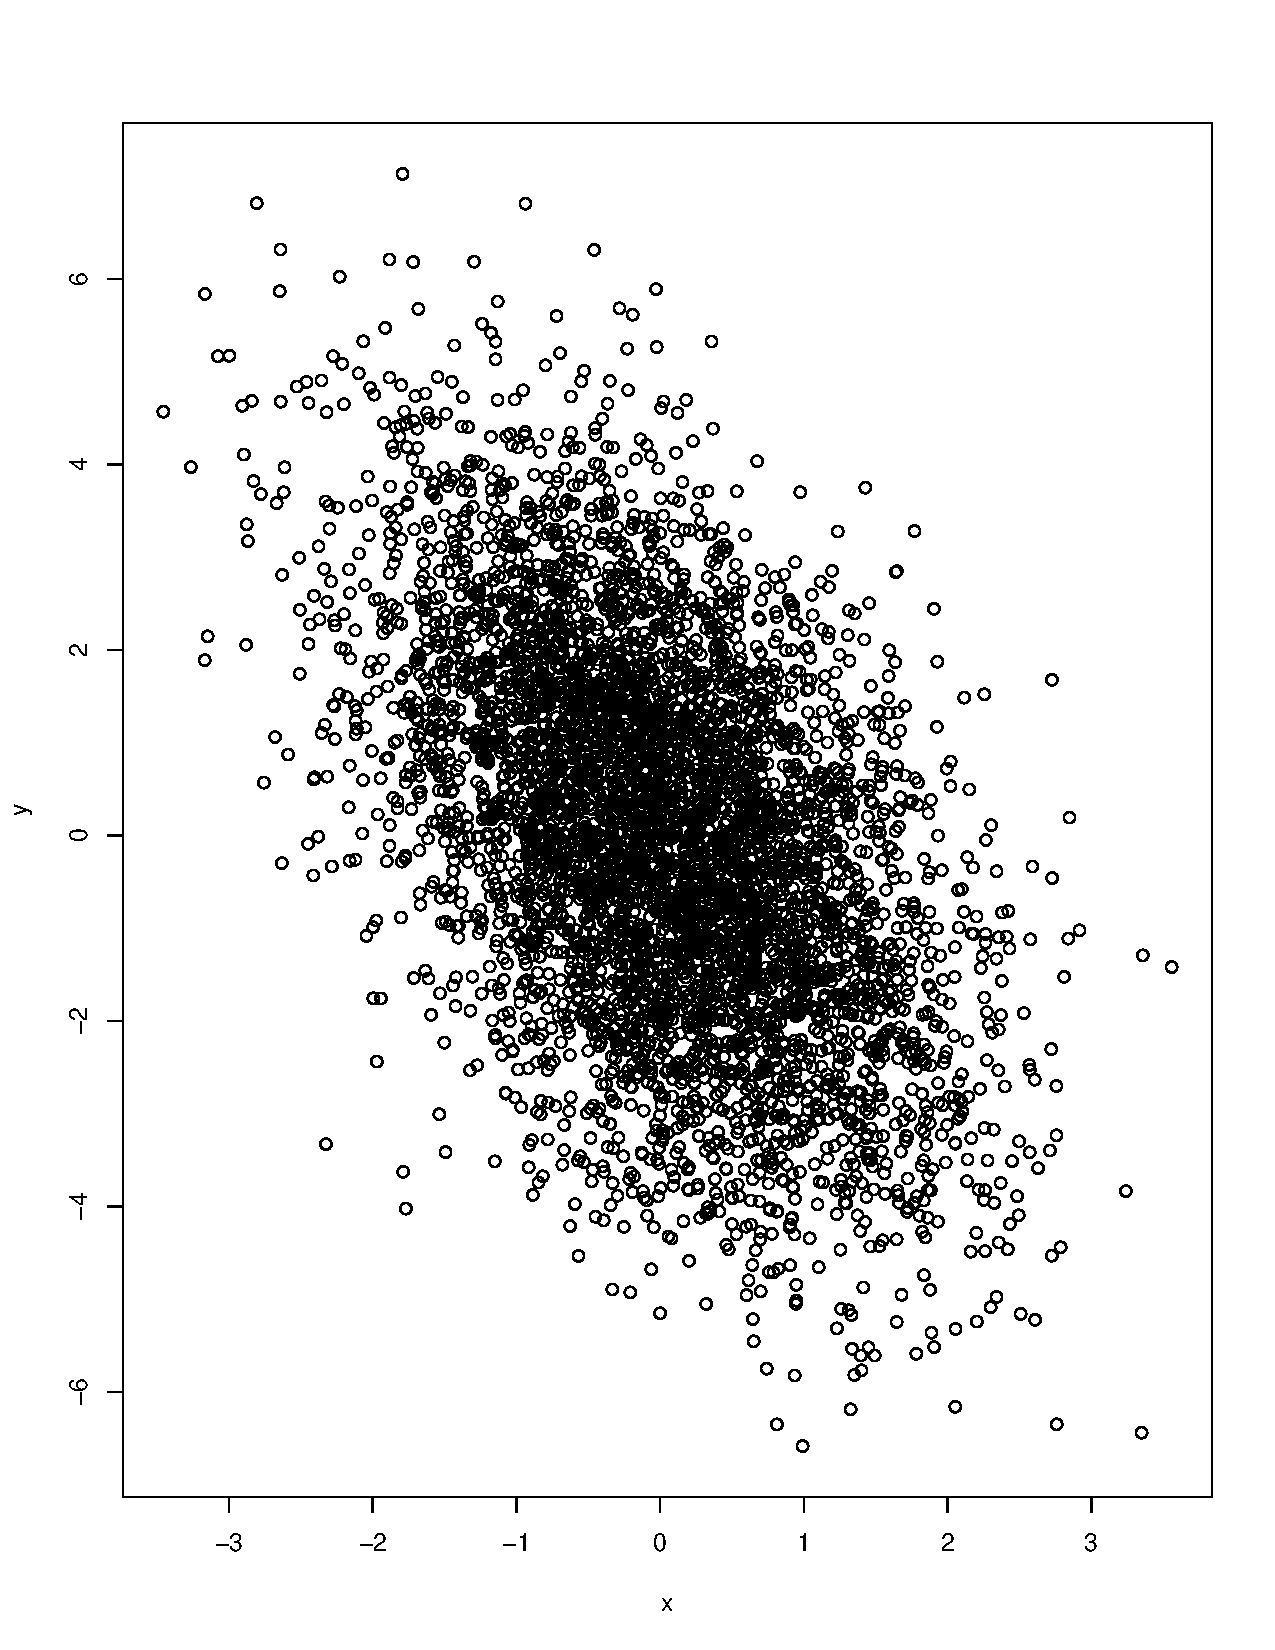
\includegraphics[width=.8\textwidth]{mvnormal_scatter.pdf}
     \end{center}
\end{column}
\end{columns}
\end{frame}


%  \begin{frame}
%\frametitle{Multivariate Normal Marginal Densities}
%\begin{center}
%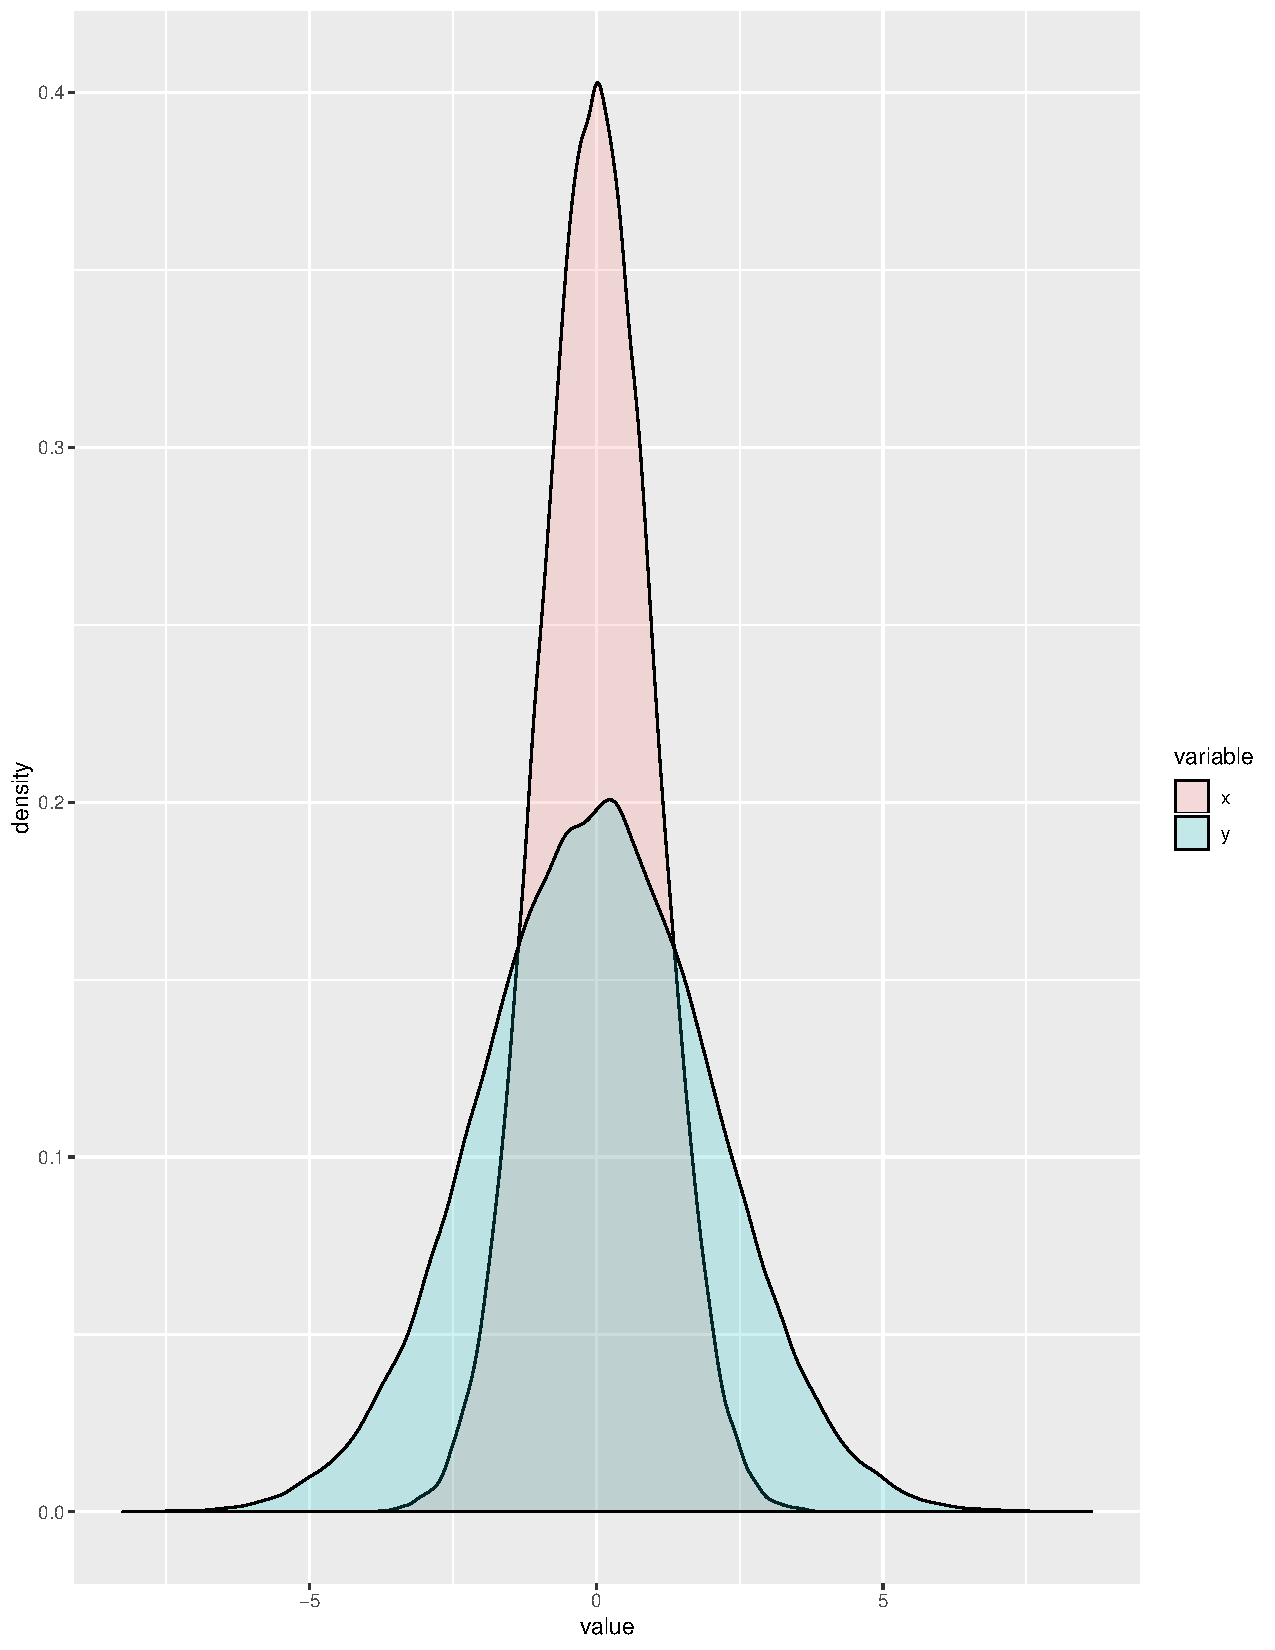
\includegraphics[scale=.25]{marginal_dists.pdf}
%\end{center}
%\end{frame}

 % \begin{frame}
%\frametitle{Multivariate Normal Marginal Densities}
%\begin{center}
%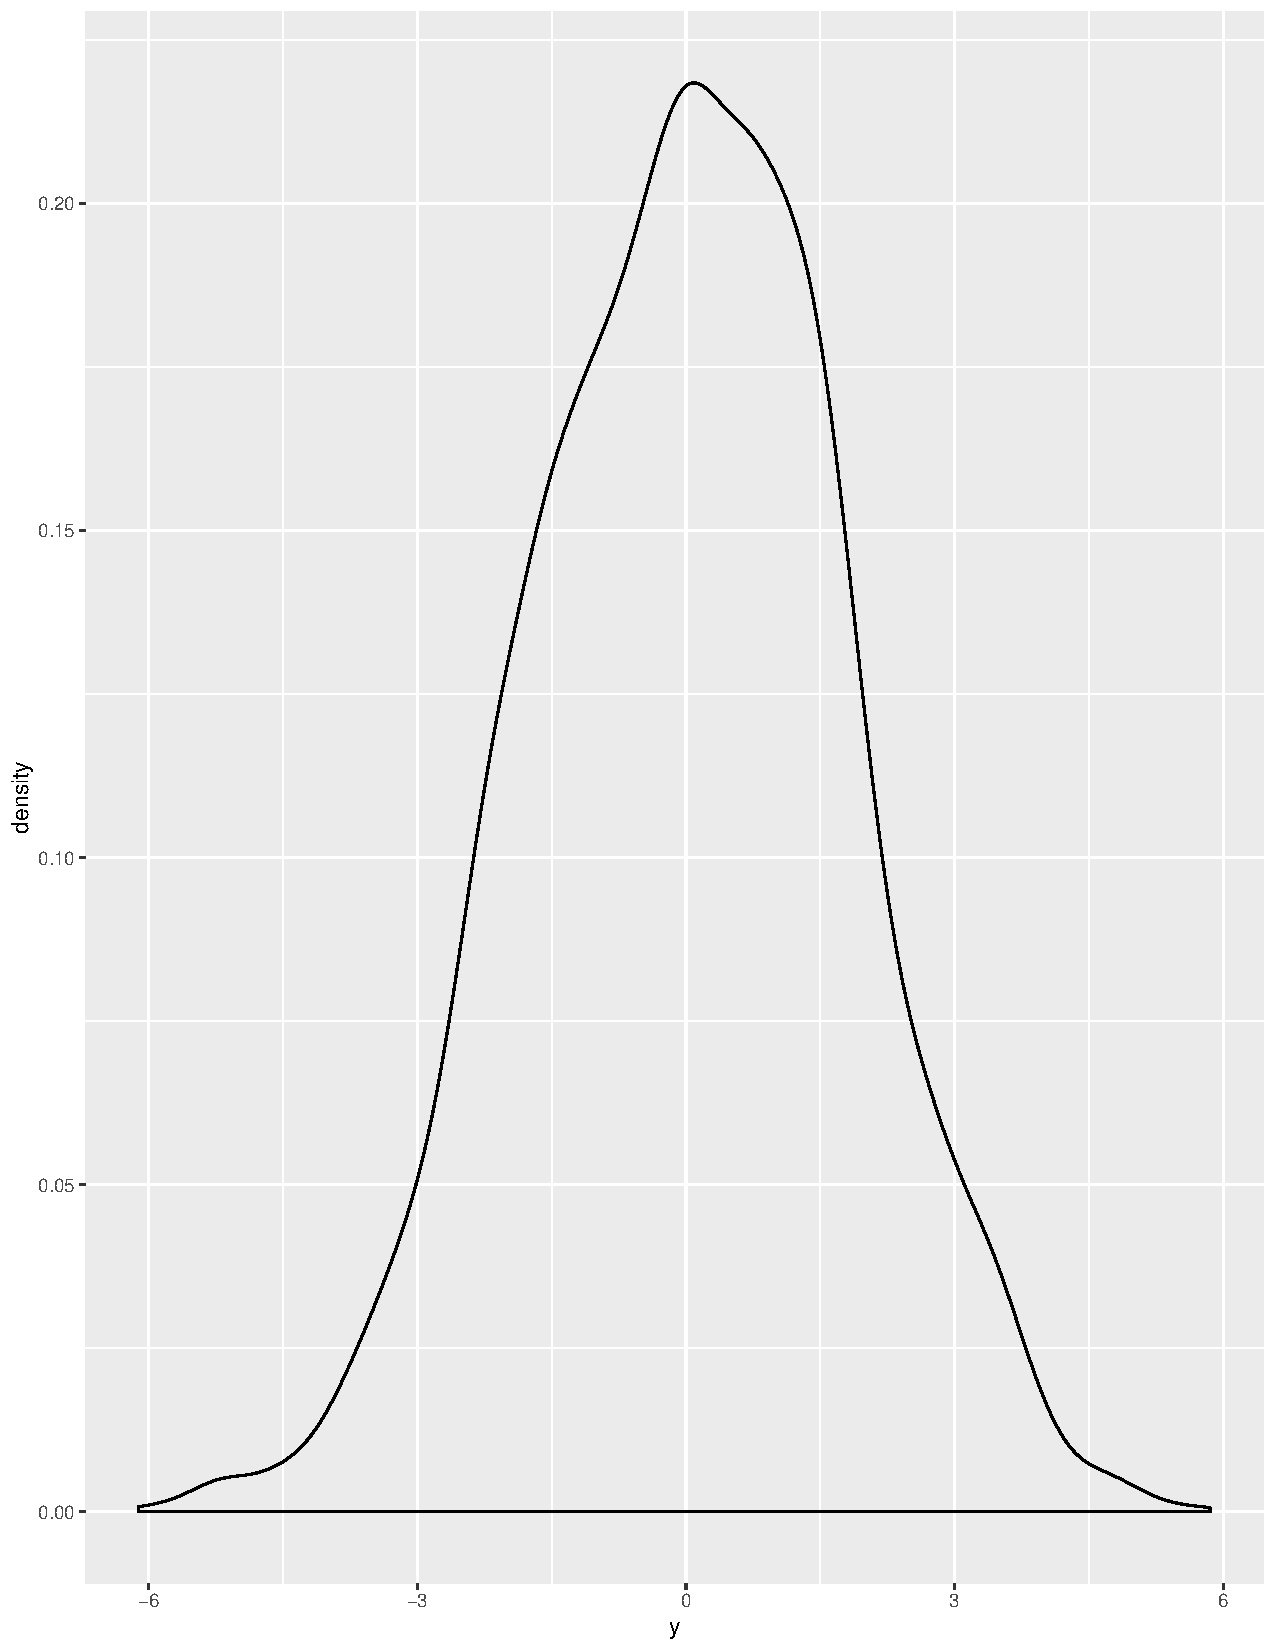
\includegraphics[scale=.2]{cond_dist.pdf}
%\end{center}
%\begin{itemize}
%	\item Here, I approximate the conditional density
%	$Pr\left(y|x=0\right)$ by plotting the density of $y$
%	when we focus on observations with $x\in\left(-.04,.04\right)$
%\end{itemize}
%\end{frame}


\begin{frame}[fragile]{ R code}
\begin{lstlisting}
# install.packages('MASS')
# install.packages('ggplot2')
# install.packages('reshape')
library(MASS)
library(ggplot2)
library(reshape)

mu <- c(0,0)
Sigma <- matrix(c(1,-1,-1,4),2,2)
xy <- mvrnorm(n = 5000, mu, Sigma)
plot(xy, xlab="x",ylab="y")

xy <- mvrnorm(n = 100000, mu, Sigma)
xy.df <- as.data.frame(xy)
names(xy.df) <- c("x", "y")
xy.stacked <- melt(xy.df)
ggplot(xy.stacked, aes(value, fill = variable)) + geom_density(alpha = 0.2)

xy.selected <- xy.df[xy.df$x>-.04  & xy.df$x<.04, ]
ggplot(xy.selected, aes(y)) + geom_density(alpha = 0.2)
\end{lstlisting}
\end{frame}


\begin{frame}{Multivariate Normal and Regression Equation}
\begin{itemize}

	\item Suppose $\left(y,x\right)' \sim \mathcal{N}\left(\mu,\Sigma\right)$, where \[
\mu=\left(\begin{array}{c}
\mu_{y}\\
\mu_{x}
\end{array}\right)\qquad\qquad\Sigma=\left(\begin{array}{cc}
\sigma_{y}^{2} & \rho\sigma_{y}\sigma_{x}\\
\rho\sigma_{y}\sigma_{x} & \sigma_{x}^{2}
\end{array}\right)
\]

	\smallskip
	\item It's also the case that \[
		E\left(y|x\right) = \mu_y + \rho\frac{\sigma_y}{\sigma_x}\left(x-\mu_x\right)
	\]
	and \[
		y = E\left(y|x\right) + \varepsilon
	\]
	with $\varepsilon$ normally distributed.

	\smallskip
	\item Normally distributed error terms: the first case we will consider (and easiest to analyze)

\end{itemize}
\end{frame}


\begin{frame}{Full Rank I}
\begin{itemize}

	\item<1-> Our next assumption is that the matrix of regressors has {\bf full rank}
	\begin{itemize}
		\item<1-> ${\bf X}$ is a $n\times K$ matrix with rank $K$.
	\end{itemize}

	\medskip
	\item<2-> A model of consumption that violates full rank:\[ 
	C = \beta_1 + \beta_2 \text{Salary} + \beta_3 \text{Nonsalary income} + \beta_4 \text{Total income} + \varepsilon
	\]

	\medskip
	\item<3-> Conditional on total income, any increase in salary must be met by a proportional decrease
	in nonsalary income

%	\medskip
%	\item<3-> Suppose we knew $\beta_4$ -- how would we be able to determine $\beta_2$ and $\beta_3$? 

\end{itemize}
\end{frame}

\begin{frame}{Full Rank II}
\begin{itemize}

	\item Consider the following model of consumption:\[ 
	C = \beta_1 + \beta_2 \text{Salary} + \beta_3 \text{Nonsalary income} + \beta_4 \text{Total income} + \varepsilon
	\]
	\smallskip
\[
	\text{Total income}  = \text{Salary} + \text{Nonsalary income},
	\]
	so\[
\begin{array}{ccl}
C & = & \beta_{1}+\left(\beta_{2}+\beta_{4}\right)\text{Salary}+\left(\beta_{3}+\beta_{4}\right)\text{Nonsalary Income}+\varepsilon\\
C & = & \beta_{1}+\widetilde{\beta}_{2}\text{Salary}+\widetilde{\beta}_{3}\text{Nonsalary Income}+0\cdot\text{Total Income}+\varepsilon
\end{array}
\]

	\smallskip
	\item Assuming $\beta_{4}\ne 0$ in the original equation, we have constructed an empirically equivalent equation with different parameters.
         That is, for this model, we have different values for ${\bold \beta }$ that are {\bf observationally equivalent}. 

\end{itemize}
\end{frame}


\begin{frame}{Full Rank III}
\begin{itemize}

	\item Exercise: suppose I wanted to build a model of the approval ratings of major party nominees 
	for US president. 

	\item I want to include the following regressors:
	\begin{itemize}
		\item Years holding elected office
		\item Age
		\item Gender
		\item Indicator variable for being married to a former president
	\end{itemize}

	\item What's the problem, assuming I have data through 2020? What about in 2025? \\ Compare to the previous case with salaries -- any difference? 



\end{itemize}
\end{frame}

\begin{frame}{Linear Independence}
\begin{itemize}

	\item Another term for the full rank assumption ($Rank\left({\bf X}\right)=K$) is {\bf linear independence}.
	 {\bf Multicollinearity} refers to a lack of linear independence. When a model has multicollinearity, we 
  	say it is {\bf not identified}. 

	\medskip
	\item Note that this is distinct from statistical independence. 

	\medskip
	\item Linear independence means that one variable cannot be algebraically predicted by others. 

	\medskip
	\item Statistical independence means that the variation in two random variables is unrelated.
	Linear independence does not imply statistical independence. Why not? Does statistical independence
	imply linear independence? 
\end{itemize}
\end{frame}


\begin{frame}{Assumptions so far}
\begin{itemize}
	\item The assumptions we have introduced so far:
\end{itemize}

\begin{align*}
\boldsymbol{y} & =  \boldsymbol{X}\boldsymbol{\beta}+\boldsymbol{\varepsilon}	& (1)\\
E\left[\boldsymbol{\varepsilon}|\boldsymbol{X}\right] & =  0						& (2) \\
Rank({\bf X}) & = K 	& (3)
\end{align*}

\begin{itemize}
	\item Note that we have not made any assumptions on the statistical properties of ${\bf X}$.
	There is no need to do so; ${\bf X}$ can be fixed or random \emph{for now}. What matters
	is the distribution of the error terms conditional on  ${\bf X}$.

	\item Not all assumptions will be maintained throughout the course (or even this lecture).
	When we consider formal results, I will be explicit about which assumptions are needed. 
	
\end{itemize}
\end{frame}

\begin{frame}{Homoscedasticity}
\begin{itemize}
	\item Another important assumption is {\bf homoscedasticity}:\[
		E\left[\boldsymbol{\varepsilon} \boldsymbol{\varepsilon}' | {\bf X} \right] = \sigma^{2} {\bf I}
	\]
	where ${\bf I}$ is a  $n \times n$ identity matrix.

	\medskip
	\item Given that $E\left[\boldsymbol{\varepsilon}|\boldsymbol{X}\right] =  0$, this means that\[
	Var\left[\boldsymbol{\varepsilon} | {\bf X} \right] = \sigma^{2} {\bf I}
	\]

	\item In words, homoscedasticity says that each error term has the same variance; i.e.,   
	the variance of $\varepsilon_i$ is not related to ${\bf x}_i$. {\bf Heteroscedastcity}
	is the alternative. Can you think of some cases of heteroscedasticity? 

	\item The assumption also rules out correlation between the error terms for different observations.
	
\end{itemize}
\end{frame}



\begin{frame}{Normal Error Terms}
\begin{itemize}
	\item A convenient assumption 
	 is that error terms are {\bf normally distributed}:\[
		\boldsymbol{\varepsilon} | {\bf X} \sim \mathcal{N}\left(0,\sigma^2 {\bf I}\right)
	\]

	\medskip
	\item Where are we going?
	\begin{itemize}
		\item This assumption will make it easy to derive normally distributed estimators (just as
			normality made the LLN and CLT easy to derive)
		\item Ultimately, the central limit theorem can be used to derive {\bf asymptotic normality}
				of estimators (that is, estimators that will be normally distributed as the sample gets large),
				so in practice it's rarely necessary to assume normal error terms. 
	\end{itemize}

\end{itemize}
\end{frame}



\begin{frame}{Residuals}
\begin{itemize}
	\item We used $\boldsymbol{\beta}$ to denote the true vector of parameters; let's use
	${\bf b}$ to denote estimates of or candidates for $\boldsymbol{\beta}$.

	\item A residual is the fitted value given a particular potential parameter vector:\[
		e_i \left({\bf b}\right) = y_i - {\bf x}_i' {\bf b}
	\]

	\item A residual captures the degree to which the linear prediction ${\bf x}_i' {\bf b}$
	explains the dependent variable $y_{i}$.
	

	\item Formally, we should think of residuals as being a function of candidate parameter
	vectors, but we will often just write $e_i$. 


	\item The vector of residuals across observations is ${\bf e} \left({\bf b}\right)$
\end{itemize}
\end{frame}


\begin{frame}{Least Squares}
\begin{itemize}
	\item It makes intuitive sense to want to find a value of ${\bf b}$
	 that makes residuals small, so that the estimated model explains the data well.

	\smallskip
	\item There are many possible ways to think about making the residuals small, but
	by far the most popular criterion is the {\bf sum of squared residuals}:\[
		SSR\left({\bf b}\right) \equiv \sum_{i=1}^{n} e_i \left({\bf b}\right)^2  =  \sum_{i=1}^{n} \left(y_i - {\bf x}_i' {\bf b}\right)^{2} = {\bf e} \left({\bf b}\right) '  {\bf e} \left({\bf b}\right)
	\]

	\smallskip
	\item The {\bf least squares estimator} minimizes the sum of squared residuals:\[
		\hat{{\bf b}}_{LS} \equiv \arg \min_{{\bf b}} SSR\left({\bf b}\right) 
	\]

	\smallskip
	\item For linear models with homoscedastic errors, the least squares estimate is typically called the
	{\bf Ordinary Least Squares} estimator.

\end{itemize}
\end{frame}



\begin{frame}{Regression with Single Variable I}
	\begin{itemize}
	
	\item Let's consider a model with only a single variable regressor (and a constant):\[
	y_i = \beta_0 + \beta_1 x_i + \varepsilon_i
	\]

	\medskip
	\item For example, we might have 
	\begin{itemize}
		\item $y_i$: Dependent Variable (e.g., test score of student $i$)
		\item $x_i$: Independent Variable (e.g., class size of student $i$)
		\item $\varepsilon_i$: regression error (e.g., noise in the model)
	\end{itemize}

%	\medskip
%	\item What this looks like in a picture (with 7 observations):
	\end{itemize}
\end{frame}


%\begin{frame}
%\begin{center}
%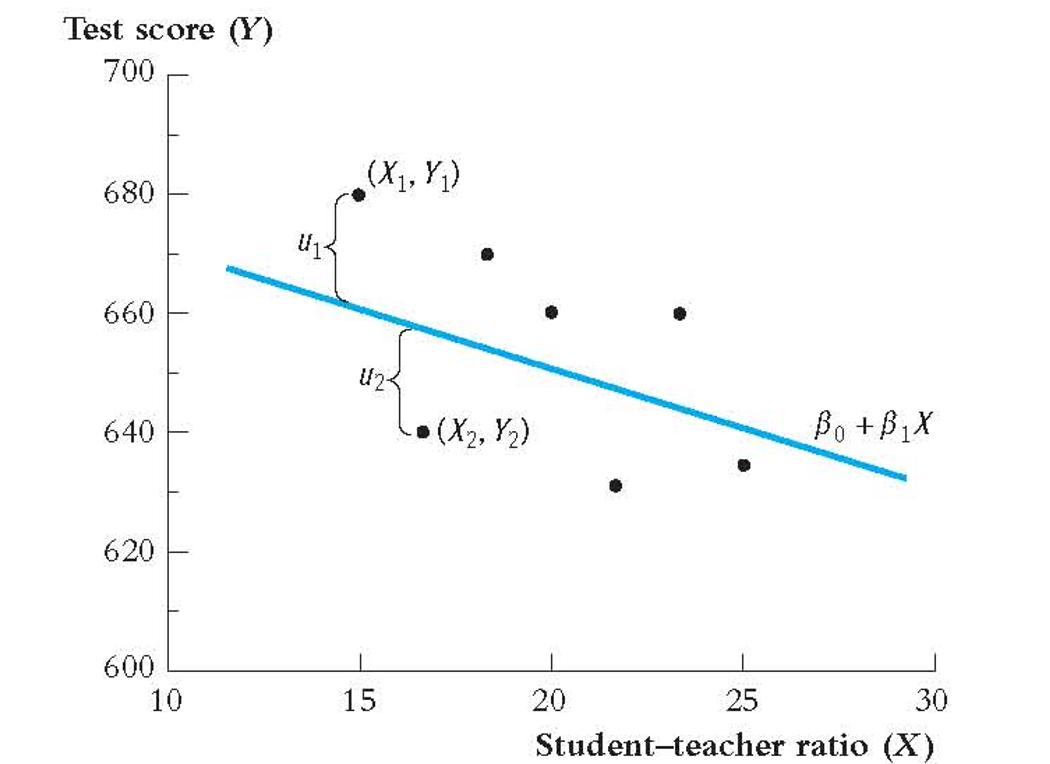
\includegraphics[width=30em]{CS_line.png}
%\end{center}
%\end{frame}


\begin{frame}{Derivation of Bivariate Linear Regression Estimator}
\[
	y_i = \beta_0 + \beta_1 x_i + \varepsilon_i
	\]

\[
		SSR\left(b_0,b_1\right) = \sum_{i=1}^{n} e_i \left(b_0,b_1\right)^2  =  \sum_{i=1}^{n} \left(y_i - b_{0} - b_{1} x_{i}\right)^{2} 
	\]


	\begin{itemize}
		\item (On board) What are the OLS estimates of $\left(\beta_0,\beta_1\right)$?
	\end{itemize}
\end{frame}

\begin{frame}{OLS Estimator}
	\begin{itemize}
\item The OLS estimates are:
\begin{align*}
\hat{b}_1 &=\frac{\sum\limits_{i=1}^n(x_i-\bar{x})(y_i-\bar{y})}{\sum\limits_{i=1}^n(x_i-\bar{x})^2}=\frac{s_{x,y}}{s_{x}^{2}} \\
\\
\hat{b}_0 & = \bar{y} - \hat{b}_1 \bar{x}
\end{align*}
where the $s_{x}^{2}$ refers to the sample variance of $x$ and $s_{x,y}$ refers to the sample covariance of $x$ and $y$.

	\end{itemize}
\end{frame}


\begin{frame}{Using the OLS Estimator}
\begin{itemize}
\item Now let's go ahead and actually use the OLS estimator.
\medskip
\item Suppose Alice has a test score of 6 and class size of 15; Bob has a test score of 3 with a class size of 20. 
\medskip
\item Our data is:
\begin{itemize}
\item Alice: $(y_1,x_1)=(6,15)$
\item Bob: $(y_2,x_2)=(3,20)$
\end{itemize}

\item Note that this is  a ridiculously small sample size (the smallest we could have and still solve for the OLS estimator). 
\end{itemize}
\end{frame}

\begin{frame}{Implementing the OLS Estimator}
\begin{itemize}
\item (On board) Find the OLS estimator for $\beta_0$ and $\beta_1$ for the data $(y_1,x_1)=(6,15)$ and $(y_2,x_2)=(3,20)$
\medskip

\item Formulas:
\begin{align*}
\hat{b}_1 &=\frac{\sum\limits_{i=1}^n(x_i-\bar{x})(y_i-\bar{y})}{\sum\limits_{i=1}^n(x_i-\bar{x})^2}=\frac{cov\left(x,y\right)}{var\left(x\right)} \\
\hat{b}_0 & = \bar{y} - \hat{b}_1 \bar{x}
\end{align*}

\item You will never have to do this algebra yourself. It becomes very cumbersome with lots of observations and with lots of regressors,
which we now turn to.

\end{itemize}
\end{frame}


\begin{frame}{Multiple Linear Regression}
\begin{itemize}
	\item Let's return to the multiple linear regression setting (multiple regressors):
	\begin{equation*}
		{\bf y}= {\bf X} \boldsymbol{\beta} + \boldsymbol{\varepsilon},
	\end{equation*}

	\item We can write the sum of squared residuals as follows:\[
	SSR\left({\bf b}\right) = {\bf e}_i \left({\bf b}\right) '  {\bf e}_i \left({\bf b}\right) = {\bf y}'{\bf y} - 2{\bf y}'{\bf X}{\bf b} + {\bf b}' {\bf X}'{\bf X}{\bf b} 
\]


	\item The necessary condition for a minimum:\[
	\frac{\partial SSR\left({\bf b}\right)}{\partial {\bf b}} = - 2 {\bf X}' {\bf y} + 2 {\bf X}'{\bf X} {\bf b} = 0 
	\]

	\item Recalling the rules:\[
\frac{\partial\boldsymbol{u}'\boldsymbol{v}}{\partial\boldsymbol{v}}=\boldsymbol{u}\qquad\qquad\frac{\partial\boldsymbol{v}'\boldsymbol{A}\boldsymbol{v}}{\partial\boldsymbol{v}}=2\boldsymbol{A}\boldsymbol{v}
\]

\end{itemize}
\end{frame}


\begin{frame}{The OLS Formula}
\begin{itemize}
	\item The necessary condition for a minimum:\[
	\frac{\partial SSR\left({\bf b}\right)}{\partial {\bf b}} = - 2 {\bf X}' {\bf y} + 2 {\bf X}'{\bf X} {\bf b} = 0 
	\]

	\item Thus, ${\bf b}$ must satisfy\[
	{\bf X}'{\bf X} {\bf b} =  {\bf X}' {\bf y} 
	\]


	\item Assuming ${\bf X}'{\bf X}$ is invertible (be careful!), we have\[
	\widehat{{\bf b}}_{OLS} \equiv  \left({\bf X}'{\bf X}\right)^{-1} {\bf X}' {\bf y} 
	\]

	\item Note the similarity to the bivariate least squares estimator. 

\end{itemize}
\end{frame}


\begin{frame}{Full Rank and Identification}
\begin{itemize}
	\item The invertibility of ${\bf X}'{\bf X}$ is not guaranteed in general, but
	it is implied by the full rank condition: $Rank\left({\bf X}\right) = K$.

	\item When ${\bf X}$ does not have full rank, neither does ${\bf X}'{\bf X}$, and \[
	{\bf X}'{\bf X} {\bf b} =  {\bf X}' {\bf y} 
	\]
	can be solved by multiple values of ${\bf b}$. 

	\item Linear algebra review: when a square matrix ${\bf A}$ is not invertible, 
	it has a non-trivial nullspace. This means that \[
	{\bf A} \boldsymbol{b} =  {\bf 0}
	\]
	can be solved by multiple vectors ${\bf b}$. This implies that, for any ${\bf c} $,
	\[
	{\bf A} {\bf b} =  {\bf c} 
	\]
	also has multiple solutions if it has at least one solution. 
	

\end{itemize}
\end{frame}


\begin{frame}{Properties of Residuals}
\begin{itemize}
	\item Let ${\bf e} $ denote the vector of OLS residuals, and consider \[
		{\bf X}' {\bf e} = {\bf X}' \left({\bf X} {\bf b}_{OLS} - {\bf y} \right) 
	\]
	\item Substituting in the OLS formula, 
 \[
		{\bf X}' {\bf e} = {\bf X}' \left({\bf X} \left({\bf X}'{\bf X}\right)^{-1} {\bf X}' {\bf y} - {\bf y} \right) 
	\]

\item This simplifies to 
 \[
		{\bf X}' {\bf e} = {\bf X}' {\bf y} -  {\bf X}' {\bf y}  = 0
	\]

	\item This implies that (1) the OLS residuals sum to zero, given that one of the regressors is a constant, and
	(2) the OLS residuals are uncorrelated with the regressors. Intuitively: there is no variation left in ${\bf e} $
	 that can be explained by ${\bf X}$.
	
\end{itemize}
\end{frame}


\begin{frame}{Method of moments preview}
\begin{itemize}
	\item Exercise: show that ${\bf b}_{OLS}$ is the unique value of $\boldsymbol{\beta}$ satisfying 
	\[
		{\bf X}' \left({\bf y} - {\bf X} \boldsymbol{\beta}  \right) =0
	\]
	given that ${\bf X}$ is full rank.

	\medskip
	\item Note that ${\bf X}$ is full rank $\Rightarrow$ ${\bf X}'{\bf X}$ is full rank.

	\medskip 
	\item Given this uniqueness result, we could use this condition to define the OLS estimator 
	instead of the least squares definition. 
	This previews {\bf method of moments} estimators, which we will discuss later.
	
\end{itemize}
\end{frame}

%\begin{frame}{Projections}
%\begin{itemize}
%	\item 
%\end{itemize}
%\end{frame}


%\begin{frame}{Idempotence}
%\begin{itemize}
%	\item 
%\end{itemize}
%\end{frame}


\begin{frame}{Multiple Regression Coefficients}
	\begin{itemize}
\item We saw that for a bivariate regression, the slope on the regressor is given by
\[
\hat{b}_1 =\frac{s_{x,y}}{s_{x}^{2}} 
\]

\medskip
\item Does it follow that, with multiple regressors, the coefficient on the $k$th regressor is
\[
\hat{b}_k =\frac{s_{x_{k},y}}{s_{x_{k}}^{2}} ?
\]

\medskip
\item If not, under what conditions?

\end{itemize}
\end{frame}


\begin{frame}{Silly Example}
	\begin{itemize}
	\item Consider the following model of rectangular painting area:\[
	\ln A_{i} = \beta_0 + \beta_{1} \ln W_{i} + \beta_{2} \ln H_{i} + \varepsilon_{i}
	\]
	where 
	\begin{itemize}
		\item $W_{i}$ is the painting $i$'s width
		\item $H_{i}$ is the painting $i$'s width
		\item $A_{i}$ is the painting $i$'s area, $A_{i} =W_{i} \cdot H_{i} $
		\item $\varepsilon_i$ is measurement error in painting $i$'s area
	\end{itemize}

	\medskip
	\item What should the $\beta$'s be in theory (i.e., given what you know about geometry)?
\end{itemize}
\end{frame}



\begin{frame}{Silly Example II}
	\begin{itemize}
	\item Suppose $\ln W_i$ and $\ln H_i$ are correlated in the population (naturally)\[
\left(\begin{array}{c}
\ln W_{i}\\
\ln H_{i}
\end{array}\right)\sim\mathcal{N\left(\left(\begin{array}{c}
\mu_w\\
\mu_h
\end{array}\right),\left(\begin{array}{cc}
\sigma_{w}^{2} & \sigma_{wh}\\
\sigma_{wh} & \sigma_{h}^{2}
\end{array}\right)\right)}
\]
	\smallskip
	\item Then, notice that\[
	\begin{array}{ll}
	Cov\left( \ln A_{i}, \ln W_{i}\right) & = Cov\left(\ln W_{i} + \ln H_{i}, \ln W_{i}\right) \\
	& = Var\left( \ln W_{i}\right) + Cov\left(\ln W_{i}, \ln H_{i}\right) 
	\end{array}
	\]

	\smallskip
	\item Finally, \[
\hspace*{-.5cm}\frac{Cov\left(\ln A,\ln W\right)}{Var\left(\ln W\right)}=\frac{Var\left(\ln W\right)+Cov\left(\ln H,\ln W\right)}{Var\left(\ln W\right)}=1+\frac{Cov\left(\ln H,\ln W\right)}{Var\left(\ln W\right)}
\]
\end{itemize}
\end{frame}


\begin{frame}{Silly Example III}
	\begin{itemize}
	\item In a bivariate regression of $A$ on $W$ (ommiting $H$), recall the slope would be given by \[
	\hspace*{-.5cm}\frac{Cov\left(\ln A,\ln W\right)}{Var\left(\ln W\right)}=1+\frac{Cov\left(\ln H,\ln W\right)}{Var\left(\ln W\right)},
	\]
	so the term $\frac{Cov\left(\ln H,\ln W\right)}{Var\left(\ln W\right)}$ represents bias. 

	\smallskip
	\item Implication: if the OLS coefficients in a multiple regression had the same formula 
	as the coefficients in a bivariate regression, there would be bias. 

	\smallskip
	\item Exception: if the regressors $\ln H$ and $\ln W$ are uncorrelated, there will be no bias above, and
	OLS with multiple regressors delivers the same coefficients as if we ran a bivariate regression with each
	of the regressors separately. 

	\smallskip
	\item This example also makes a point about omitted variables bias: if height is unobserved, the regression
	of $\ln A$ on only $\ln W$ will deliver the biased coefficient above.
	
\end{itemize}
\end{frame}

\begin{frame}{Silly Example IV}

	\[
	\widehat{{\bf b}}_{OLS} \equiv  \left({\bf X}'{\bf X}\right)^{-1} {\bf X}' {\bf y} 
	\]


	\begin{itemize}
	\item Indeed, OLS with multiple regressors does not deliver 
	the bivariate regression coefficient $s_{x_{k}y}/s_{x_{k}}^{2}$ for each regressor $x_{k}$
	(except in the case of orthogonal regressors)

	\bigskip
	\item To gain some intuition for what this formula is doing, let's consider the $ \left({\bf X}'{\bf X}\right)$
	and ${\bf X}' {\bf y} $ pieces separately in the context of the silly model of painting area.


\end{itemize}
\end{frame}






\begin{frame}{Silly Example V}


	\begin{itemize}
	\item Suppose that $w_{i}=\ln W_{i}-\mu_{w}$ and $\ln h_{i}=\ln H_{i}-\mu_{h}$


	\item Let $\boldsymbol{X}=\left[\boldsymbol{w}\quad\boldsymbol{h}\right]$

	\item It follows that 
\[
\boldsymbol{X}'\boldsymbol{X}=\left(\begin{array}{cc}
\sum\left(\ln W_{i}-\mu_{w}\right)^{2} & \sum\left(\ln W_{i}-\mu_{w}\right)\left(\ln H_{i}-\mu_{h}\right)\\
\sum\left(\ln W_{i}-\mu_{w}\right)\left(\ln H_{i}-\mu_{h}\right) & \sum\left(\ln H_{i}-\mu_{h}\right)^{2}
\end{array}\right)
\]
Note: if we multiply that by $n^{-1}$, we have the sample analog of the
covariance matrix. 
	
\end{itemize}
\end{frame}

\begin{frame}{Silly Example VI}

	\begin{itemize}
	\item Similarly,
\[
\boldsymbol{X'}\boldsymbol{y}=\left(\begin{array}{c}
\sum\left(\ln W_{i}-\mu_{w}\right)\left(\ln A_{i}-\mu_{a}\right)\\
\sum\left(\ln H_{i}-\mu_{h}\right)\left(\ln A_{i}-\mu_{a}\right)
\end{array}\right),
\]
is the sample covariance of $\boldsymbol{x}$ and $\boldsymbol{y}$
(times $n$). 

\smallskip
\item Therefore, we have
\[
\widehat{\boldsymbol{b}}_{OLS}=\left(\boldsymbol{X}'\boldsymbol{X}\right)^{-1}\boldsymbol{X}'\boldsymbol{y}=\left(n^{-1}\boldsymbol{X}'\boldsymbol{X}\right)^{-1}\left(n^{-1}\boldsymbol{X}'\boldsymbol{y}\right)=S_{xx}^{-1}s_{xy}
\]
where $S_{xx}$ is the sample covariance matrix for $\boldsymbol{x}$
and $s_{xy}$ is the sample covariance of $\boldsymbol{x}$ and $y$. 

\end{itemize}
\end{frame}


\begin{frame}{Silly Example VII}

\[
\widehat{\boldsymbol{b}}_{OLS}=S_{xx}^{-1}s_{xy}
\]

\begin{itemize}
	\item The population moments for the model of painting areas are \[
Var\left(\boldsymbol{x}\right)=\left(\begin{array}{cc}
\sigma_{w}^{2} & \sigma_{wh}\\
\sigma_{wh} & \sigma_{h}^{2}
\end{array}\right)\qquad\qquad Cov\left(\boldsymbol{x},y\right)=\left(\begin{array}{c}
\sigma_{w}^{2}+\sigma_{wh}\\
\sigma_{h}^{2}+\sigma_{wh}
\end{array}\right)
\]

\item Note that 
\[
\left(Var\left(\boldsymbol{x}\right)\right)^{-1}=\frac{1}{\sigma_{w}^{2}\sigma_{h}^{2}-\sigma_{wh}^{2}}\left(\begin{array}{cc}
\sigma_{h}^{2} & -\sigma_{wh}\\
-\sigma_{wh} & \sigma_{w}^{2}
\end{array}\right)
\]

\item With some algebra, the population-moments version of OLS gives us the right coefficients:
\[
\left(Var\left(\boldsymbol{x}\right)\right)^{-1}Cov\left(\boldsymbol{x},y\right)=\left(\begin{array}{c}
1\\
1
\end{array}\right)
\]
\end{itemize}
\end{frame}







\begin{frame}{The Frisch-Waugh Theorem I}
\begin{itemize}
	\item Think about separating $ {\bf X}$ into two sub-matrices:\[
	 {\bf X} =  \left[{\bf X}_{1}\quad  {\bf X}_2 \right],
	\]
	with \[
	{\bf y} = {\bf X}_{1} \boldsymbol{\beta}_{1} +  {\bf X}_{2} \boldsymbol{\beta}_{2} + \boldsymbol{\varepsilon}
	\]
\end{itemize}

\begin{block}{Frisch-Waugh Theorem}
The OLS regression of ${\bf y} $ on $\left[{\bf X}_{1},  {\bf X}_2 \right]$
yields a subvector ${\bf b}_{2}$ of coefficient estimates that is the same as
the result from a regression of the residuals from a regression
of ${\bf y} $ on ${\bf X}_{1}$ are regressed on the residuals
from a regression of ${\bf X}_{2}$ on ${\bf X}_{1}$.

\end{block}
\end{frame}

\begin{frame}{The Frisch-Waugh Theorem II}
\begin{itemize}
	\item In other words, let's start by regressing ${\bf y} $ on ${\bf X}_{1}$.
	Let's label the residuals from this regression ${\bf y}^{*} $.

	\item Let's also regress ${\bf X}_{2}$ on ${\bf X}_{1}$ 
	(think about regressing each column of ${\bf X}_{2}$ on ${\bf X}_{1}$).
	Let's label the residuals from this regression ${\bf X}^{*}_{2}$.

	\item If we regress ${\bf y}^{*}$ on ${\bf X}^{*}_{2}$, we get the same
	coefficient on ${\bf X}^{*}_{2}$ that we would have had in the full
	regression of  ${\bf y} $ on $\left[{\bf X}_{1},  {\bf X}_2 \right]$.

	\item An implication is that
	the coefficient on each variable can be thought of as the effect
	of that variable after controlling for all the other variables. Thus,
	OLS coefficients are sometimes called {\bf partial regression coefficients}.

\end{itemize}
\end{frame}



\begin{frame}{The Frisch-Waugh Theorem III}
\begin{itemize}
	\item Bivariate linear regression is easy to visualize (scatter plot with a line running through).
	Frisch-Waugh tells us how we can visualize the effect of a single variable from a multiple
	regression.

	\medskip
	\item One implication of Frisch-Waugh is that, if we de-mean all the variables and then 
	run a regression with the de-meaned variables (but leaving out the constant term in ${\bf X}$),
	we will get the same coefficients on all the variables.
	\begin{itemize}
		\item Exercise: given the Frisch-Waugh theorem, show this formally. 
	\end{itemize}
\end{itemize}
\end{frame}



\begin{frame}{Units and Coefficients}
\begin{itemize}
	\item Recalling that $E\left[{\bf y}|{\bf X}\right] = {\bf X} \boldsymbol{\beta}$, a natural interpretation	of
	the coefficients is 
	is \[
	\beta_1 = \frac{d }{d X_{1i}}E\left[y_i |{\bf X}\right]
	\]
	
	\item In simple linear regression, it's easy to see that re-scaling (changing the units
	of $x$) will rescale the parameter estimates in the opposite way:\[
		\hat{b}_1 =\frac{\sum\limits_{i=1}^n(x_i-\bar{x})(y_i-\bar{y})}{\sum\limits_{i=1}^n(x_i-\bar{x})^2}
	\]
 	The same is true in the multiple regression framework (Frisch-Waugh makes this easier to see). 

	\medskip
	\item Exercise: if the regressor $x$ in a bivariate regression
	is the log of a variable, show that rescaling the original variable does not
	affect $\hat{b}_1 $. What about $\hat{b}_0$? 
\end{itemize}
\end{frame}




\begin{frame}{Goodness of Fit}
\begin{itemize}
	\item The {\bf total sum of squares}, or the {\bf total variation} in the dependent variable:\[
	SST = \left({\bf y} - {\bf i} \overline{y} \right)' \left({\bf y} - {\bf i} \overline{y} \right)
	\]

	\smallskip
	\item The dependent variable decomposes into a prediction and a residual:\[
	{\bf y} = {\bf X} {\bf b} + {\bf e} =  \widehat{{\bf y}} + {\bf e}
	\]
where ${\bf X} {\bf b} =  \widehat{{\bf y}}$ is the prediction or {\bf fitted value} of $y$. 

	\smallskip
	\item We can think about decomposing the variation in $y$ into variation in $ \widehat{{\bf y}}$ and ${\bf e}$.
	Intuitively, we want the variation in  $ \widehat{{\bf y}}$ to account for as much as possible
\end{itemize}
\end{frame}



\begin{frame}{Sums of Squares}
\begin{itemize}
	\item Define \[
\boldsymbol{M}_{0}=I-n^{-1}\boldsymbol{1}\boldsymbol{1}'.
\]
note that $\boldsymbol{M}_{0}$ is symmetric and {\bf idempotent}.

\smallskip
\item Notice that $ {\bf y}'\boldsymbol{M}_{0}{\bf y}$ is the SST. 

\smallskip
\item Also, we can show that
\[
\boldsymbol{y}'\boldsymbol{M}_{0}\boldsymbol{y}=\boldsymbol{b}'\boldsymbol{X}'\boldsymbol{M}_{0}\boldsymbol{X}\boldsymbol{b}+\boldsymbol{e}'\boldsymbol{e},
\]
where the first term on the RHS is known as the \textbf{regression
sum of squares (SSR)}, and the second term is the \textbf{error sum
of squares (SSE)}.\[
SST = SSR + SSE
\]
	
\end{itemize}
\end{frame}

\begin{frame}{Coefficient of Determination}
\begin{itemize}
	\item The coefficient of determination is defined as the proportion of the variation in the dependent variable
	explained by the model:\[
	R^{2} = \frac{SSR}{SST} =  \frac{\boldsymbol{b}'\boldsymbol{X}'\boldsymbol{M}_{0}\boldsymbol{X}\boldsymbol{b}}{\boldsymbol{y}'\boldsymbol{M}_{0}\boldsymbol{y}}
	= 1 -  \frac{{\bf e}'{\bf e}}{\boldsymbol{y}'\boldsymbol{M}_{0}\boldsymbol{y}}
\]

	\smallskip
	\item $R^{2}$ is a measure of goodness of fit that always goes up as we add more regressors. It doesn't 
	tell us whether it's ``worth it'' to add a new regressor to the model. (Later we will talk about why overfitting
	can be bad in finite samples.)

\smallskip
	\item {\bf Adjusted} $R^{2}$ incorporates a penalty for the number of regressors:
	\[
	\overline{R}^{2} 	= 1 -  \frac{{\bf e}'{\bf e}/\left(n-K\right)}{\boldsymbol{y}'\boldsymbol{M}_{0}\boldsymbol{y}/\left(n-1\right)}
	\]
\end{itemize}
\end{frame}




\begin{frame}{Finite Sample Properties}
\begin{itemize}
	\item Given assumptions (1)-(3), homoscedasticity, and normal error terms, \[
	{\bf b}_{OLS} | {\bf X} \sim \mathcal{N}\left(\boldsymbol{\beta},\sigma^{2} \left({\bf X}'{\bf X}  \right)^{-1} \right)
	\]





	\item Proof on board

	\item Note: proof that it's unbiased and expression for variance
	do not require normally error terms, but it would be hard to say what the finite sample
	distribution is, exactly, without normality. 

\end{itemize}
\end{frame}




\begin{frame}{Standard Errors}

\[
	{\bf b}_{OLS} | {\bf X} \sim \mathcal{N}\left(\boldsymbol{\beta},\sigma^{2} \left({\bf X}'{\bf X}  \right)^{-1} \right)
	\]

\begin{itemize}
	\item $\sigma^{2} \left({\bf X}'{\bf X}  \right)^{-1}$ is the covariance matrix of the parameter estimates
	-- it tells us how precise ${\bf b}_{OLS}$ is as an estimate of $\boldsymbol{\beta}$.

	\item The diagonal elements of $\sigma^{2} \left({\bf X}'{\bf X}  \right)^{-1}$ are the variances of each of
	the parameter estimates. The square roots of those are {\bf standard errors}. Note that standard
	errors are standard deviations of the distribution of an estimator. 

	\item The off-diagonal elements of $\sigma^{2} \left({\bf X}'{\bf X}  \right)^{-1}$ are also important
	(especially when we get to hypothesis testing).
	They indicate whether two parameter estimates are correlated.

\end{itemize}
\end{frame}

\begin{frame}{Estimating Standard Errors}

\[
	{\bf b}_{OLS} | {\bf X} \sim \mathcal{N}\left(\boldsymbol{\beta},\sigma^{2} \left({\bf X}'{\bf X}  \right)^{-1} \right)
	\]

\begin{itemize}
	\item $\left({\bf X}'{\bf X}  \right)^{-1}$ is just data, but $\sigma^{2}$ must be estimated (recall that it's the 
	variance of the normally distributed error terms). 

	\item Intuitively, the residuals are estimates of the error terms, so the sample variance of residuals
	is what we use to estimate $\sigma^{2}$:\[
	s^{2} = \frac{{\bf e}'{\bf e}}{n-K}
	\]

	\item Similar to how the unbiased estimator of the variance of a random variable with unknown mean requires us to divide
	by $n-1$, here we have to divide by $n-K$, where $K$ is the number of parameters being estimated. 

	
\end{itemize}
\end{frame}


\begin{frame}{Mean-squared error}
\begin{itemize}
	\item Consider a parameter vector $\boldsymbol{\gamma}$ and consider
	${\bf x}'\boldsymbol{\gamma}$ as a predictor of $y$. 

	\medskip
	\item The {\bf mean squared error} of this predictor is\[
	MSE = E\left[\left( y - {\bf x}' \boldsymbol{\gamma}\right)^{2}\right]
	\]

	\item This can be written\[
	MSE = E\left[ \left(y - E\left[y | {\bf x}\right]\right)^{2}\right] + E\left[  \left(E\left[y | {\bf x}\right]- {\bf x}' \boldsymbol{\gamma}\right)^{2} \right]
	\]
	(check this by expanding and applying the law of iterated expectations)

	\item Result: OLS is the value of $\boldsymbol{\gamma}$ that minimizes mean square error. This does not
	require normality of the error terms. (Proof on board)
	
\end{itemize}
\end{frame}


\begin{frame}{Gauss-Markov Theorem}

\begin{block}{Gauss-Markov Theorem}
In the linear regression model with homoscedastic errors, The OLS estimator 
is the {\bf best linear unbiased estimator} (BLUE).
\end{block}

\begin{itemize}
	\item ``Best'' means estimator with lowest variance -- most precise

	\item Normally distributed error not assumed here

	\item If error terms are not homoscedastic, OLS is still unbiased given strict
	exogeneity, but lower-variance estimators are possible (see: Generalized Least Squares)

	\item Proof on board
	
\end{itemize}
\end{frame}


\begin{frame}{Generalized Least Squares}
\begin{itemize}
	\item The proof that OLS is unbiased did not rely on homoskedasticity. OLS
	is ``LUE'' even without homoskedasticity. OLS is only {\bf B}LUE (minimal variance) with homoskedasticity.

	\smallskip
	\item Without homoskedasticity, but maintaining our other assumptions, {\bf Generalized
		Least Squares} is BLUE. That is, suppose,\[
	Var\left[\boldsymbol{\varepsilon} | {\bf X} \right] = \boldsymbol{\Omega}
	\]
	then the BLUE estimator is \[
	{\bf b}_{GLS} = \left({\bf X}'\boldsymbol{\Omega}^{-1}{\bf X}\right)^{-1} {\bf X}' \boldsymbol{\Omega}^{-1}{\bf y} .
	\]
	
	\smallskip
	\item To implement GLS, note that $\boldsymbol{\Omega}$ must be estimated ({\bf Feasible Generalized
		Least Squares}). In contrast, OLS estimates the $\boldsymbol{\beta}$ parameters without needing to know or estimate
		anything about variances; $\sigma^2$ is only needed to quantify standard errors. 
\end{itemize}
\end{frame}



\begin{frame}{Endogeneity}
\[
	{\bf b}_{OLS} = \left({\bf X}'{\bf X}\right)^{-1} {\bf X}' {\bf y} = \boldsymbol{\beta}  + \left({\bf X}'{\bf X}\right)^{-1} {\bf X}' \boldsymbol{\varepsilon}
	\]
\begin{itemize}
		\item Note that our argument for OLS being unbiased involved a step where we argue that \[
	E\left[\left({\bf X}'{\bf X}\right)^{-1} {\bf X}' \boldsymbol{\varepsilon}\right] =0
	\]
	thanks to strict endogeneity.

	\medskip
	\item If one of the regressors is correlated with $\varepsilon$, strict exogeneity is violated, and this term will cause bias. 

\end{itemize}
\end{frame}


\begin{frame}{Omitted Variables Bias}
\begin{itemize}
	\item Suppose the econometrician only observes regressors ${\bf X} $, but the true model is\[
			{\bf y}= {\bf X} \boldsymbol{\beta} + {\bf z} \gamma + \boldsymbol{\varepsilon},
	\]

	\item The OLS estimator will equal\[
	{\bf b} = \left({\bf X}'{\bf X}\right)^{-1} {\bf X}' {\bf y} = \boldsymbol{\beta}  + \left({\bf X}'{\bf X}\right)^{-1} {\bf X}' {\bf z} \gamma + \left({\bf X}'{\bf X}\right)^{-1} {\bf X}' \boldsymbol{\varepsilon}
	\]

	\item The last term is mean zero given the strict exogeneity assumption.

	\item Note that the second term will not be zero if ${\bf X}$ and ${\bf z}$ are correlated;
	i.e. if $ {\bf X}' {\bf z} \ne 0$.

	\item Implication:  correlation between omitted variables and the observed regressors makes OLS biased.

	
\end{itemize}
\end{frame}







\begin{frame}{Bias with multiple variables}
\begin{itemize}
		\item<1-> Consider a model with two variables:\[
			y_i = \beta_0 + \beta_1 x_{1,i} + \beta_2 x_{2,i} + \varepsilon_i,
		\]
		and suppose that
		\begin{align*}
			x_{1,i} =& u_{1,i} + u_{3,i} + \varepsilon_i  \\
			x_{2,i} =& u_{2,i} + u_{3,i}
		\end{align*}		
		where the $u$'s and $\varepsilon$ are all independently distributed. 
		
		\item<1-> We know that OLS will deliver
		a biased estimate of $\beta_{1}$, but will OLS still be consistent for $\beta_2$?
		
		\medskip
		\item<2-> No! The correlation between $x_1$ and $x_2$ leads to bias even
		in $\beta_2$.
		\begin{itemize}
			\item<2-> Thus, endogeneity problems are a big deal not only for our variables of interest; endogenous
			control variables can also create problems.
		\end{itemize}
\end{itemize}
\end{frame}


\begin{frame}{Bias with multiple variables II}
\begin{itemize}
		\item Consider ``controlling'' for $x_1$ with the wrong estimate $b_1$ of $\beta_1$:\[
					y_i - b_1 x_{1,i} = \beta_0 + \beta_2 x_{2,i}  + \varepsilon_i + (\beta_1 - b_1) x_{1,i},
\]

\medskip
		\item Given that $b_1 \ne \beta_1$, we get some stuff in the error term:\[
					y_i - b_1 x_{1,i} = \beta_0 + \beta_2 x_{2,i}  + \varepsilon_i + (\beta_1 - b_1) (u_{1,i} + u_{3,i} + \varepsilon_i),
\]
and we now have an endogeneity problem because $x_{2,i} = u_{2,i} + u_{3,i}$ and $u_{3,i}$ is now in the error term.

\medskip
\item Note: we could formalize this intuition using the Frisch-Waugh Theorem. 
\end{itemize}
\end{frame}


\begin{frame}{Irrelevant Variables}
\begin{itemize}
	\item What if we include a variable in ${\bf X}$ that doesn't actually
	affect $y$?

	\smallskip
	\item This can be accommodated in the linear regression framework as
	a regressor that has a coefficient $\beta_{k}=0$.

	\smallskip
	\item Thus, this does not create any bias in the other coefficients, and the 
	expected coefficient on the irrelevant variable is zero.

	\smallskip
	\item However, this can reduce the precision of the estimates of the 
	other coefficients, and it's not generally a good idea to add as many variables
	to a regression as you can ({\bf overfitting}). More on this later. 

	
\end{itemize}
\end{frame}




\begin{frame}{Finite Sample vs. Asymptotic Properties}
\begin{itemize}
	\item It's rare to have small-sample properties of an estimator

	\medskip
	\item Econometric studies typically do Monte Carlo (simulation) studies to learn
	about finite-sample performance of estimators. 

	\medskip
	\item For most estimators, we derive asymptotic properties, i.e., \[
	\sqrt{n} \left({\bf b}_{OLS} - \boldsymbol{\beta}\right) \Rightarrow_{d} \mathcal{N}\left(0, \Sigma\right)
	\]

	\item The above statement says that the OLS estimator
	 {\bf converges in distribution} to a normally distributed variable.

	\item Part of that result is that OLS is {\bf consistent}. Formally, consistency means that an estimator
	{\bf converges in probability} to the true value. 
\end{itemize}
\end{frame}



\begin{frame}{Asymptotics: Setup}
\begin{itemize}

	\item Asymptotic analysis refers to analyzing statistics of the data as the number of observations $n$
	grows to infinity (e.g., the central limit theorem).

	\item To do asymptotic analysis, we specify a {\bf data generating process}. 
	
	\item A data generating process describes the distribution of 
	 a sequence of observations $\left(\boldsymbol{x}_{i},\varepsilon_{i}\right)$ 	for $i=1,2,\dots n$. 


	\item The simplest case is assuming that observations are {\bf independent and identically distributed}
	(i.i.d)

	\item In other settings, the observations are allowed to be correlated, but in a limited way 
	that requires the dependence between ``distant'' observations to go to zero -- see {\bf stationarity}
	and {\bf ergodicity} (e.g., time series, and 	more recently some spatial analysis)

	\item We also need the data to be ``well-behaved'', i.e. $E\left[{\bf x} {\bf x}' \right]$ must have
	full rank and the error terms must have finite variance. 

\end{itemize}
\end{frame}



\begin{frame}{OLS Asymptotic Distribution}
\begin{itemize}
	\item We can use the central limit theorem to show that OLS is asymptotically
	normally distributed:\[
\boldsymbol{b}_{OLS}\sim^{a}\mathcal{N}\left(\boldsymbol{\beta},\frac{\sigma^{2}}{n}E\left[\boldsymbol{x}_{i}\boldsymbol{x}_{i}'\right]^{-1}\right)
\]
	where $ \sim^{a}$ signifies convergence in distribution. 

	\item This is just like the finite-sample distribution
	we got with normally distributed error terms. 
\end{itemize}
\end{frame}





\end{document}